%----------------------------------------------------------------
%
%  File    :  chapter6.tex
%
%  Authors : Michael Fuska, FH Campus Wien, Austria
%  Created : 13 Feb 2016
%
%  Changed :  
% 
%----------------------------------------------------------------


\chapter{Analyse und Ergebnisse}
\label{ch:Ergebnisse}

%------------------------------------------------------------------------------
%------------------------------ Analysen zur Frage 1

\section{Welche Faktoren sind für die Sicherheit und die Vertrauenswürdigkeit eines iOS Device ausschlaggebend?}
\label{sec:Frage1}

\begin{table}[htp!]
    \begin{center}
        \begin{tabular}{|p{30mm}|p{27mm}|p{13mm}|p{10mm}|p{18mm}|p{2cm}|p{15mm}|} \hline
            \textbf{iOS Device} & \textbf{Verkaufsstart} & \textbf{initiale iOS} & \textbf{letzte iOS} & \textbf{Secure Enclave} & \textbf{Prozessor}  & \textbf{\#Tage JB} \\ \hline
            \textbf{iPhone} & 29.06.2007  & 1.0 & 3.1.3 & nA & Samsung SSL8900 & 11\\ \hline
            \textbf{iPhone 3G} & 11.07.2008 & 2.0 & 4.2.1 & nA & Samsung SSL8900 & 9\\ \hline
            \textbf{iPhone 3GS} & 19.06.2009 & 3.0 & 6.1.6 & nA & Samsung SSL8920 & 14\\ \hline
            \textbf{iPhone 4} & 01.08.2010 & 4.0 & 7.1.2 & nA & Apple A4 & 38 \\ \hline
            \textbf{iPhone 4s} & 20.01.2012 & 5.0 & 9.3.2 & nA & Apple A5 & 98 \\ \hline 
            \textbf{iPhone 5} & 21.09.2012 & 6.0 &  9.3.2 & nA & Apple A6 & 136 \\ \hline
            \textbf{iPhone 5c} & 22.12.2013 & 7.0 & 9.3.2 & nA & Apple A6 & 93 \\ \hline
            \textbf{iPhone 5s} & 22.12.2013 & 7.0 & 9.3.2 & A & Apple A7 & 93 \\ \hline
            \textbf{iPhone 6} & 19.09.2014 & 8.0 & 9.3.2 & A & Apple A8 & 33\\ \hline
            \textbf{iPhone 6 Plus} & 19.09.2014 & 8.0 & 9.3.2 &  A & Apple A8 & 33\\ \hline
            \textbf{iPhone 6s} & 25.09.2016 & 9.0 &  9.3.2 & A & Apple A9 & 19\\ \hline
            \textbf{iPhone 6s Plus} & 25.09.2016 & 9.0 & 9.3.2 &  A & Apple A9 & 19\\ \hline
            \textbf{iPhone SE} & 31.03.2016 & 9.0 &  9.3.2 & A & Apple A9 & nA\\ \hline  
        \end{tabular} 
        \caption{Auflistung iOS Device/ Verkaufsstart/ initiale iOS Version / letzte unterstützte iOS Version / Prozessor/ \# JB Veröffentlichungstage \protect\footnotemark}
        \label{tab:iOSHW}
    \end{center}
\end{table}
\footnotetext{Quelle Eigenwerk}

In der Tabelle \ref{tab:iOSHW} werden alle iOS Devices aufgelistet und in Verbindung zum Verkaufszeitpunkt des Device, der initial installierten iOS Version und des Prozessor-Typs des iDevice gebracht. Zusätzlich wird in der Tabelle angeführt, ob diesem Device ein Coprozessor mit Secure Enclave zur Verfügung steht und wie lange die JB-Community benötigt, um ein JB für dieses Device zu veröffentlichen. Diese Tabelle beinhaltet alle Daten, die als Grundlage für alle weiteren Analysen in diesem Kapitel dienen.\par


%------------------------------------------------------------------------------
%------------------------------ 
\subsection{iOS Device (G1.1)}
\label{sec:Frage1iOSDevice} 

Die Tabelle \ref{tab:iOSHW} alleine gibt noch keinen Aufschluss über den Zusammenhang zwischen der Sicherheit des Systems und der verwendeten iOS Hardware. Zudem lässt Tabelle \ref{tab:iOSHW} keine Aussagen darüber zu, ob der Zeitraum bis zum Veröffentlichen des JB nur von der iOS Hardware abhängt oder von der iOS Version, die am Device installiert wurde. Aus diesem Grund müssen die Daten der beiden Tabellen (Tab. \ref{tab:iOSHW}, Tab. \ref{tab:iOSVersion}) korreliert werden. \par 
\begin{table}[htp!]
    \begin{center}
        \begin{tabular}{|l|l|l|} \hline
         \textbf{iOS Version} & \textbf{veröffentlicht am} & \textbf{\#Tage JB}\\ \hline    
        1.0 & 29.06.2007 & 11\\ \hline 
        2.0 & 11.07.2008	& 9\\ \hline 
        3.0 & 17.06.2009	& 2\\ \hline 
        4.0 & 21.06.2010 & 2\\ \hline 
        5.0 & 12.10.2011	& 1\\ \hline 
        6.0 & 19.09.2012	& 0\\ \hline 
        7.0 & 18.09.2013	& 95\\ \hline 
        7.1-7.1.2 & 29.05.2014 & 25\\ \hline 
        8.0 & 17.09.2014	& 35\\ \hline 
        8.1.1-8.4 & 17.11.2014	& 12\\ \hline 
        9.0 & 16.09.2015	& 28\\ \hline
       %  9.0.1 & 23.09.2015 & nA \\ \hline
       %  9.0.2 & 30.09.2015 & nA \\ \hline 
        9.1 & 21.10.2015	& 142\\ \hline 
       %  9.2 & 08.12,2015 & nA\\ \hline
       % 9.2.1 & 18.02.2016 & nA \\ \hline
       %  9.3 & 21.03,016 & nA\\ \hline 
       % 9.3.1 & 31.03.2016 & nA\\ \hline
       % 9.3.2 & 17.05.2016 & nA \\ \hline
        \end{tabular} 
        \caption{Auflistung iOS Version/ iOS Veröffentlichungsdatum/ \# Tage bis zur Veröffentlichung des JB \protect\footnotemark}
        \label{tab:iOSVersion}
    \end{center}
\end{table}
\footnotetext{Quelle Eigenwerk}

Die Tabelle \ref{tab:iOSVersion} listet die iOS Version, das Veröffentlichungsdatum dieser, sowie die Anzahl an Tagen die benötigt wurden, um einen JB für diese iOS Version zu veröffentlichen, auf.  \par 
Die Abbildung \ref{fig:VergleichJBProzessorSW} stellt die Verbindung zwischen den Prozessoren des iDevices, der installierten iOS Version und der benötigten Tage für die Veröffentlichung eines JB her. Es kann gezeigt werden, dass alle Apple Prozessorarchitekturen einschließlich des Apple A6 ein Sicherheitsgewinn für die iOS Produkte bedeutet haben. Dieser Schluss ist darauf begründet, dass die JBs für die selbe iOS Version auf älteren Apple Prozessorarchitekturen innerhalb von wenigen Tagen verfügbar waren. \par 

Eine Veränderung in den Daten ist ab dem Apple A7 Prozessor sichtbar. Es stellt sich lediglich ein marginaler Unterschied im Veröffentlichungszeitraum des JBs, zwischen der iOS Hardware und iOS Version, dar.

\newpage
\begin{figure}[htbp!]
        \centering
                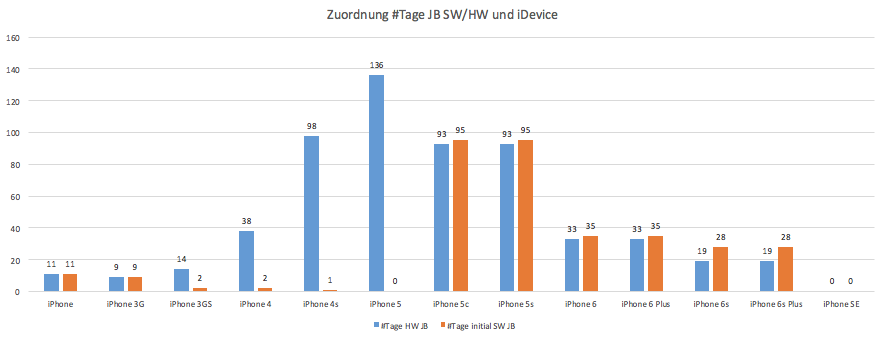
\includegraphics[scale=0.5]{Bilder/iDeviceJB-SW-HW.png}
         \caption{Vergleich Veröffentlichungstage eines JB für die Prozessoren und deren initiale iOS Version \protect\footnotemark}
        \label{fig:VergleichJBProzessorSW}      
\end{figure}
\footnotetext{Quelle Eigenwerk}

\paragraph{Ergebnis:} Es zeigt sich, dass die Sicherheit und die Vertrauenswürdigkeit der iOS Produkte zum heutigen Zeitpunkt nur mehr von Apples mobilen Betriebssystem abhängt und nicht von der verwendeten iOS Hardware. 
% TODO
%64 BIT Architektur
%
%------------------------------------------------------------------------------
%------------------------------ 
\subsection{Secure Enclave  (G1.1)}
\label{sec:Frage1SecureEnclave}
 
 Unter iOS gibt es die Möglichkeit, verschiedene Passcode Konfigurationen vorzunehmen. Abhängig davon, welche Prozessorgeneration verwendet wird, werden die Konfiguration und Daten des Passcodes in einer \textbf{Secure Enclave} oder im Flash Memory gespeichert. Neben der Anzahl der Stellen kann auch konfiguriert werden, ob nur Zahlen oder auch alphanumerische Werte für einen Passcode verwendet werden.\par 
 Ein weiterer iOS Konfigurationsparameter ermöglicht es, das Device so zu konfigurieren, dass nach zehn falschen Passcode Eingaben alle Daten des Gerätes gelöscht werden. Die Anzahl der Fehlversuche wird bei iOS Devices ohne Secure Enclave in den Flash Memory geschrieben. Bei iOS Devices mit Secure Enclave werden diese Daten in der \textit{\glqq ARM Trust Zone\grqq{}} gespeichert und können somit nicht ohne weiters ausgelesen und überschrieben werden. 
 
% Die Secure Enclave des Coprozessor (siehe Tabelle: \ref{tab:iOSHW}) bringen einen massiven Sicherheitsgewinn für die iOS Produkte mit sich, da die  
 
 Im Fall \textit{\glqq FBI gegen Apple\grqq{}} wurde der Tatsache, dass das iOS Device keine Secure Enclave enthält, besondere Bedeutung beigemessen. Das FBI beauftragte ein Unternehmen, um das iPhone 5c des San-Bernadino-Attentäters zu entsperren. Die Abbildung: \ref{fig:iOSSecurityArchitekturiOS7} zeigt die iOS Sicherheitsarchitektur des iPhone 5c. Die Systemarchitektur dieses iOS Device beinhaltet keine Secure Enclave. \par 
\newpage
\paragraph{Der Sicherheitsforscher Zdziarski beschreibt in seinen Abhandlungen die plausiblen Varianten des FBI Hacks wie folgt}
\begin{quote}
\begin{enumerate}
    \item \textit{\glqq .... based on all of this, is that an external forensics company, with hardware capabilities, is likely copying the NAND storage off the chip and frequently re-copying all or part of the chip’s contents back to the device in order to brute force the pin – and may or may not also be using older gear from iOS 8 techniques to do it. The two weeks the FBI has asked for are not to develop this technique (it’s most likely already been developed, if FBI is willing to vacate a hearing over it), but rather to demonstrate, and possibly sell, the technique to FBI by means of a field test on some demo units.\grqq{}} \cite{Hacking[6]} 
    \item \textit{\glqq If the FBI did in fact use a software exploit, the question then becomes one of how viable it is on other platforms. Typically, a software exploit of this magnitude could very well take advantage of vulnerabilities that have long existed in the firmware, making it more than likely that the exploit may also be effective (possibly with a little tailoring) to older versions of iOS. Even if the exploit today was tailored specifically for this device, adjusting offsets and patching slightly different copies of Apple’s firmware is a relatively painless process. A number of open source tools even exist to find and patch the correct bytes in decrypted Apple kernels.\grqq{}} \cite{Hacking[7]}
\end{enumerate}
  
\end{quote}
\paragraph{Ergebnisse:} Die Secure Enclave bietet einen Sicherheitsgewinn für die iOS Produkte, aber der Fall \textit{\glqq FBI via Apple\grqq{}} lässt einige Fragen offen. Da das FBI Apple die Sicherheitslücke nicht offenlegte, gibt es nur Mutmaßungen, über den Hack der verwendet wurde, um das iPhone des Attentäters zu entsperren. \par 

Zdziarski beschreibt die möglichen Folgen dieses Hacks wie folgt: 
\begin{quote}
    \textit{\glqq The moral of the story is that the exploit the FBI may have is dangerous in and of itself, regardless of whether it serves their specific purposes of brute forcing a device’s pin. Such an exploit has numerous uses within the intelligence community and poses a threat to not only the hundreds of millions of older devices out there, but if it can be ported to a 64-bit platform, every single one of us – either directly as a threat from the government, a nation state the exploit developer also sold it to, or another hacker who finds the same hole because FBI didn’t report the vulnerability to Apple. FBI has left us all potentially exposed by choosing to keep their technique secret.\grqq{}} \cite{Hacking[4]} \par 
\end{quote}
Vor allem gibt es Vermutungen, dass der Hack des FBIs eine Möglichkeit bietet, die Secure Enclave zu umgehen.


\newpage
%------------------------------------------------------------------------------
%------------------------------ 
\subsection{iOS Version  (G1.2)}
\label{sec:Frage1iOSVersion} 

\begin{figure}[hp!]
        \centering
                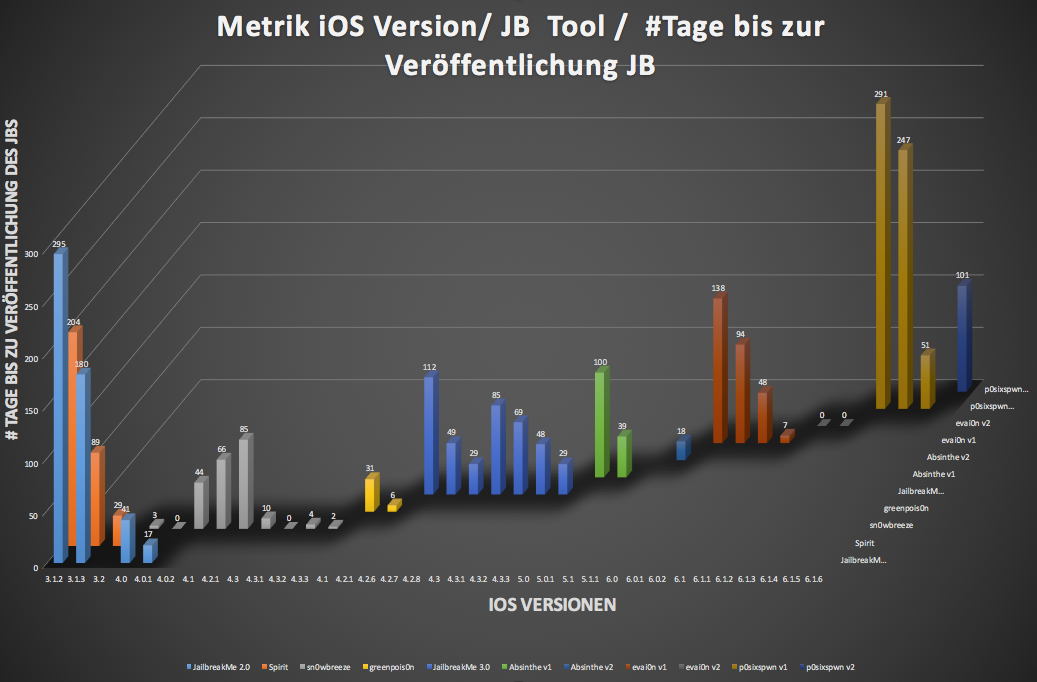
\includegraphics[scale=0.45]{Bilder/Frage1_1.png}
        \caption{Auflistung iOS Version 3.x - 4.x / JB Tools / \newline \# Veröffentlichungstage JB \protect\footnotemark}
        \label{fig:AnalyseiOSJB1}        
\end{figure}
\footnotetext{Quelle Eigenwerk}

\begin{figure}[htbp!]
        \centering
                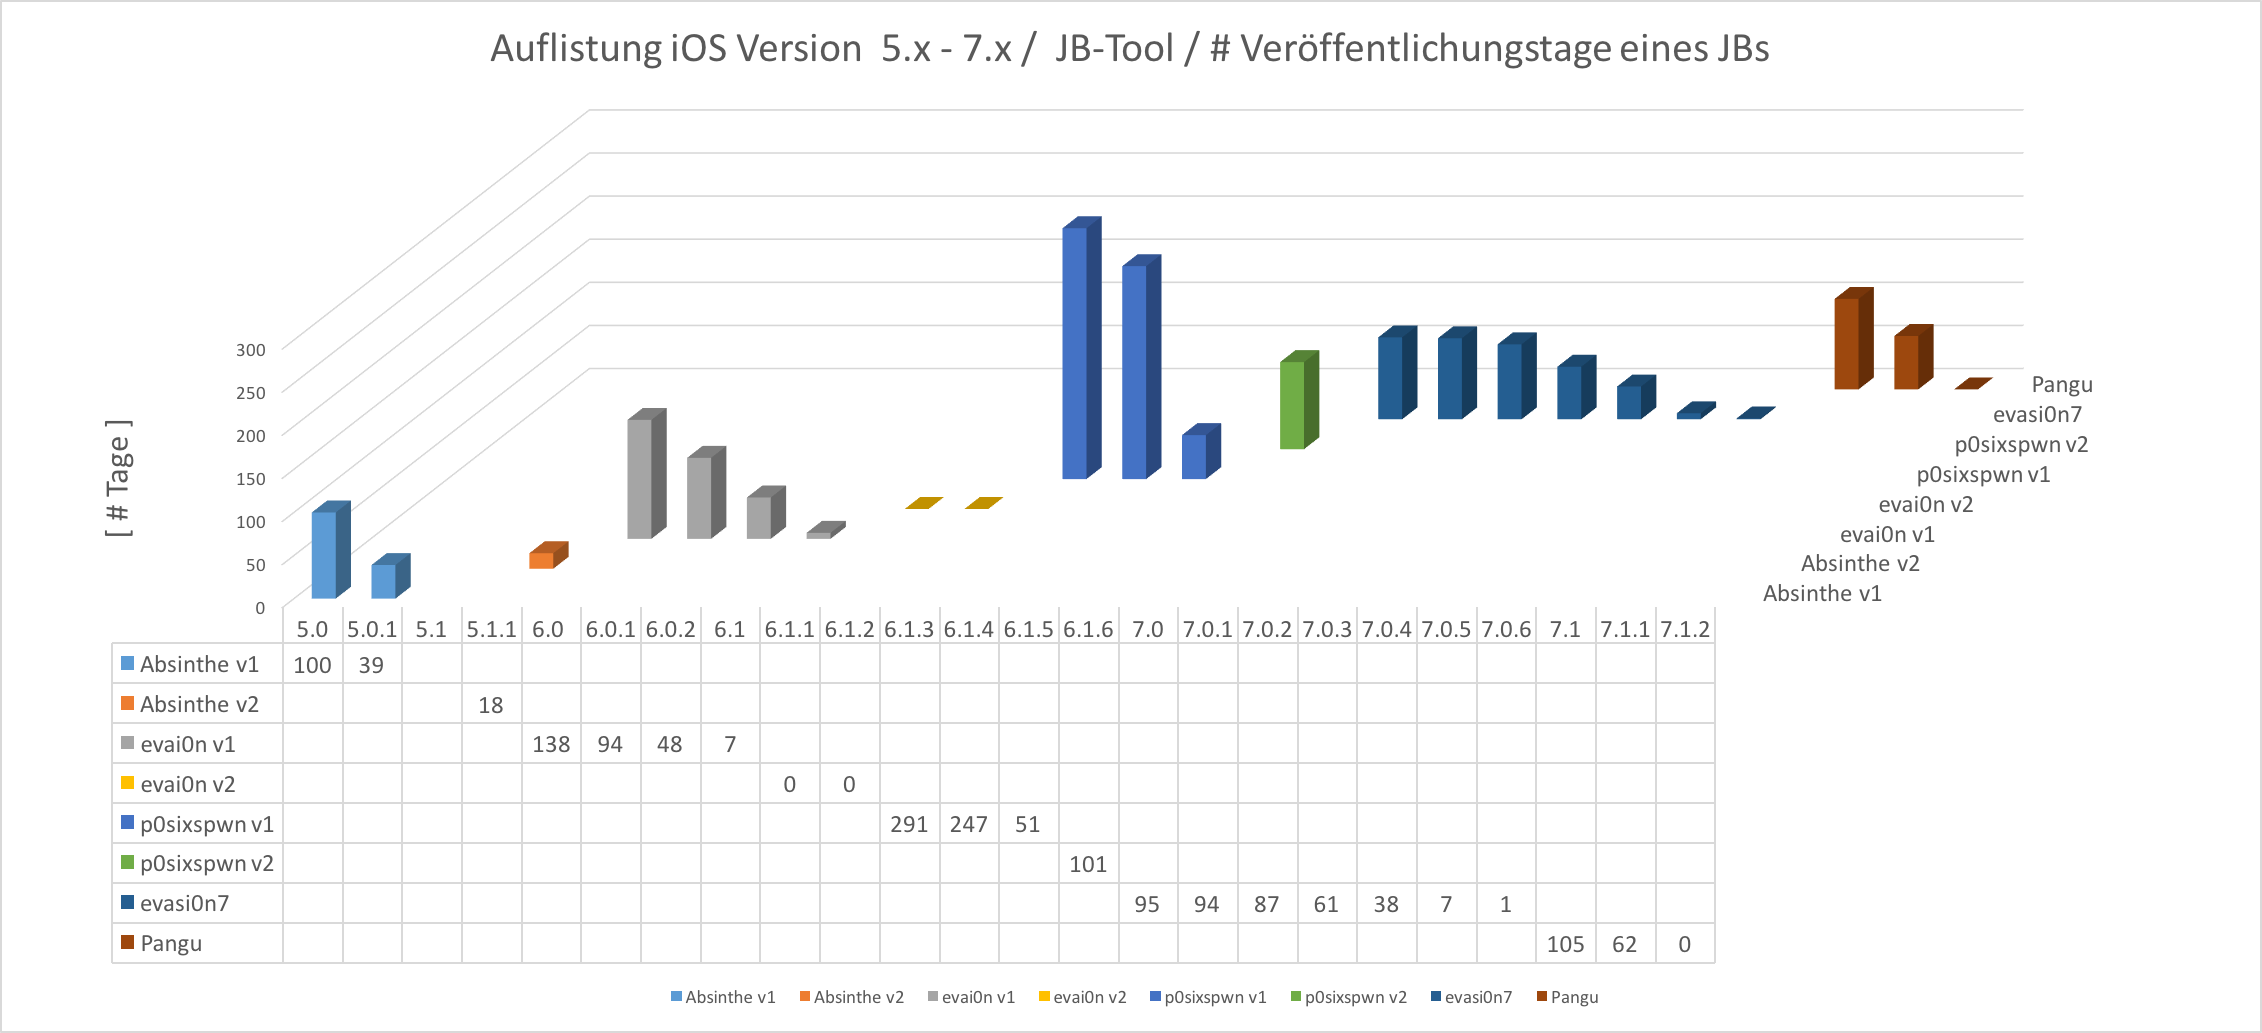
\includegraphics[scale=0.45]{Bilder/Frage1_2.png}
        \caption{Auflistung iOS Version 5.x - 7.x/ JB Tools / \newline \# Veröffentlichungstage JB \protect\footnotemark}
        \label{fig:AnalyseiOSJB2}
\end{figure}
\footnotetext{Quelle Eigenwerk}
\newpage

\begin{figure}[htbp!]
        \centering
                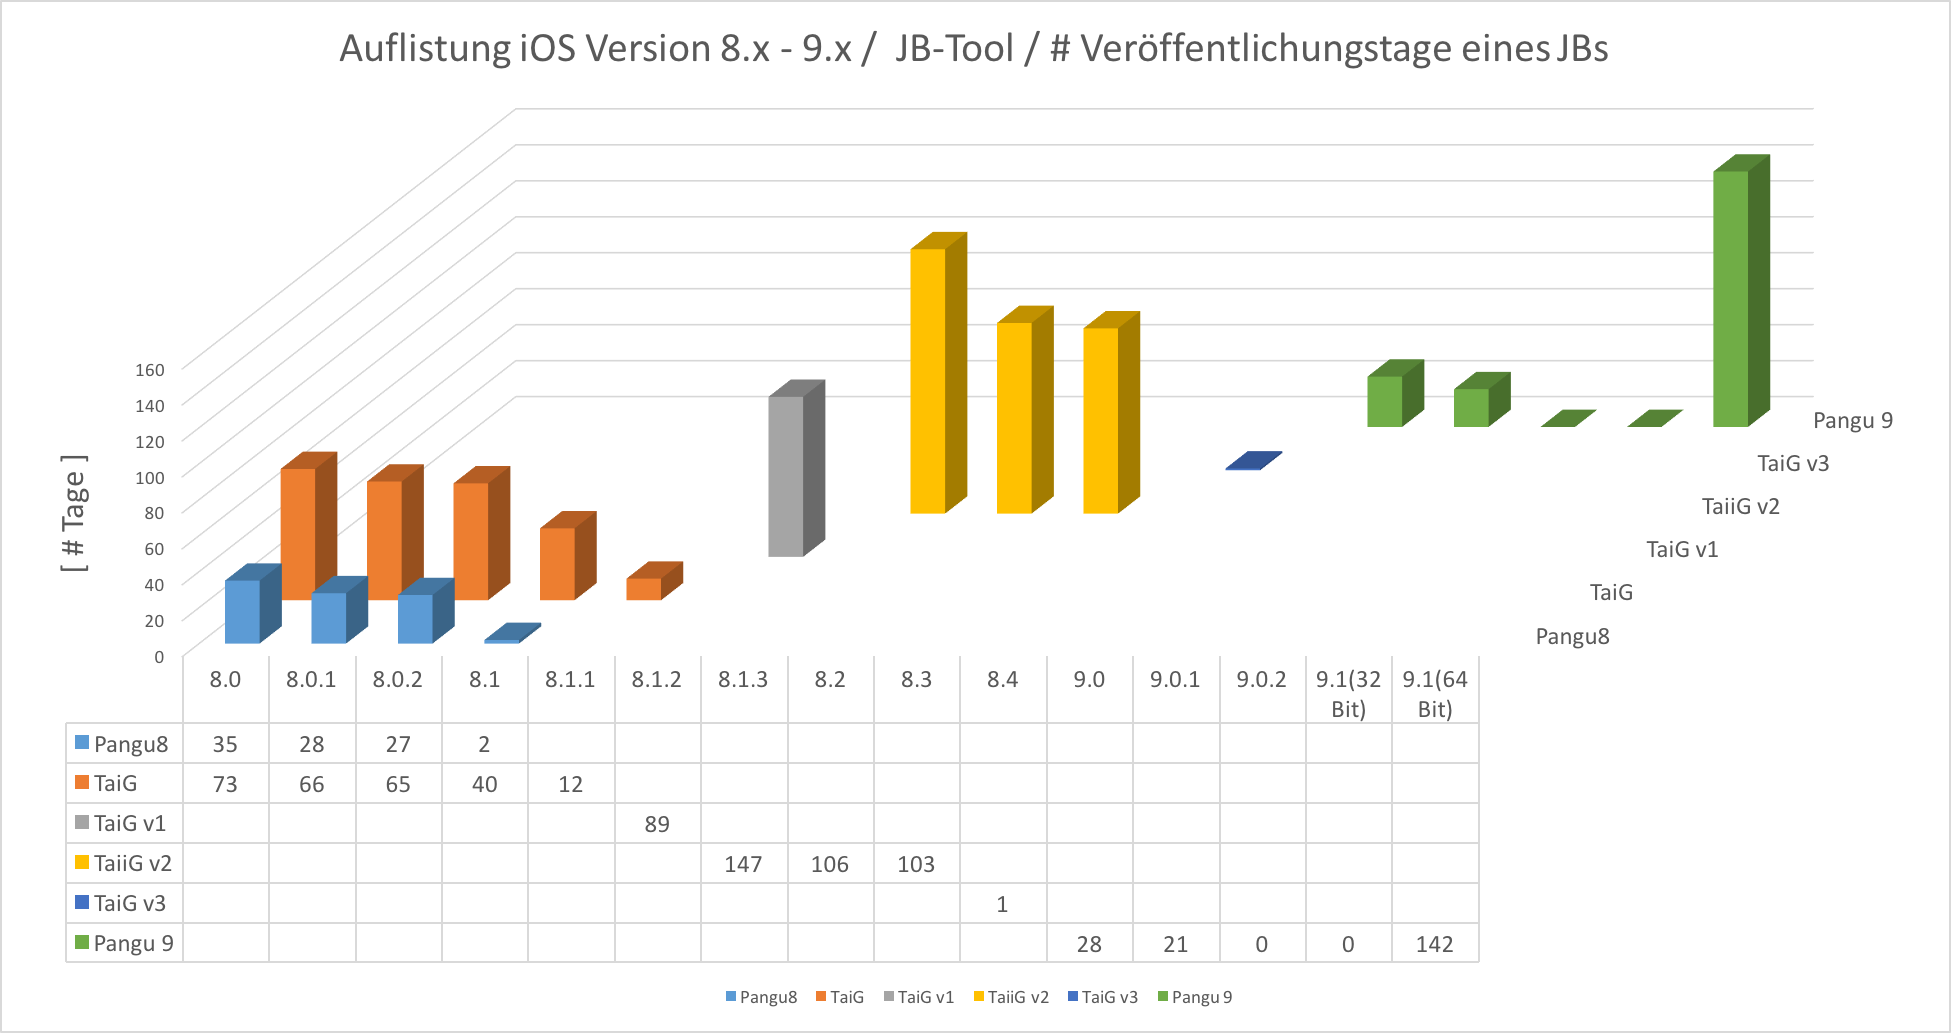
\includegraphics[scale=0.5]{Bilder/Frage1_3.png}
        \caption{Auflistung iOS Version 8.x - 9.x/ JB Tools / \newline \# Veröffentlichungstage JB \protect\footnotemark}
        \label{fig:AnalyseiOSJB3}
\end{figure}
\footnotetext{Quelle Eigenwerk}
Die Abbildungen \ref{fig:AnalyseiOSJB1}, \ref{fig:AnalyseiOSJB2} und \ref{fig:AnalyseiOSJB3} zeigen die bekanntesten und stabilsten untethered JBs, in Abhängigkeit mit der iOS Version und der Anzahl an Tagen, die benötigt wurden, um für diese iOS Version einen Jailbreak bereitzustellen. \par 
\textbf{Die Graphiken zeigen,} dass ein JB immer nur bei einer Serie von iOS Versionen funktioniert. In den meisten Fällen funktioniert der JB für die \textit{\glqq aktuelle\grqq{}} iOS Version und einigen iOS Versionen davor. Nach wenigen Wochen stellt Apple ein iOS Sicherheitsupdate zur Verfügung, welches das JB verhindert. Dieses Verhalten zieht sich durch alle betrachteten Metriken.  
%
%dass nach einem gelungen JB die Sicherheitsupdates von Apple einen kurzzeitigen Sicherheitsmehrwert mit sich bringen, aber innerhalb einiger Tage wurde ein neuer JB, des selben JB-Team veröffentlicht. Dies lässt darauf schliessen, dass die Sicherheitslücken nur teilweise geschlossen worden sind. Dieser Verhalten gilt  für alle iOS Versionen bis einschliesslich der iOS Version 9.x.\par  
%Ab der iOS Version 8.x ändert sich dieses Verhalten, da die JB Community jetzt länger für die JBs der nachfolgenden iOS minor Releases benötigt. \par 
%Markant ändern sich die Muster ab der iOS Version 9.x. Das JB für die Minor iOS Version 9.1 benötigte fast sechsmal länger, als das JB für die Major iOS Version 9.0 benötigte.\par

\begin{figure}[htbp!]
        \centering
                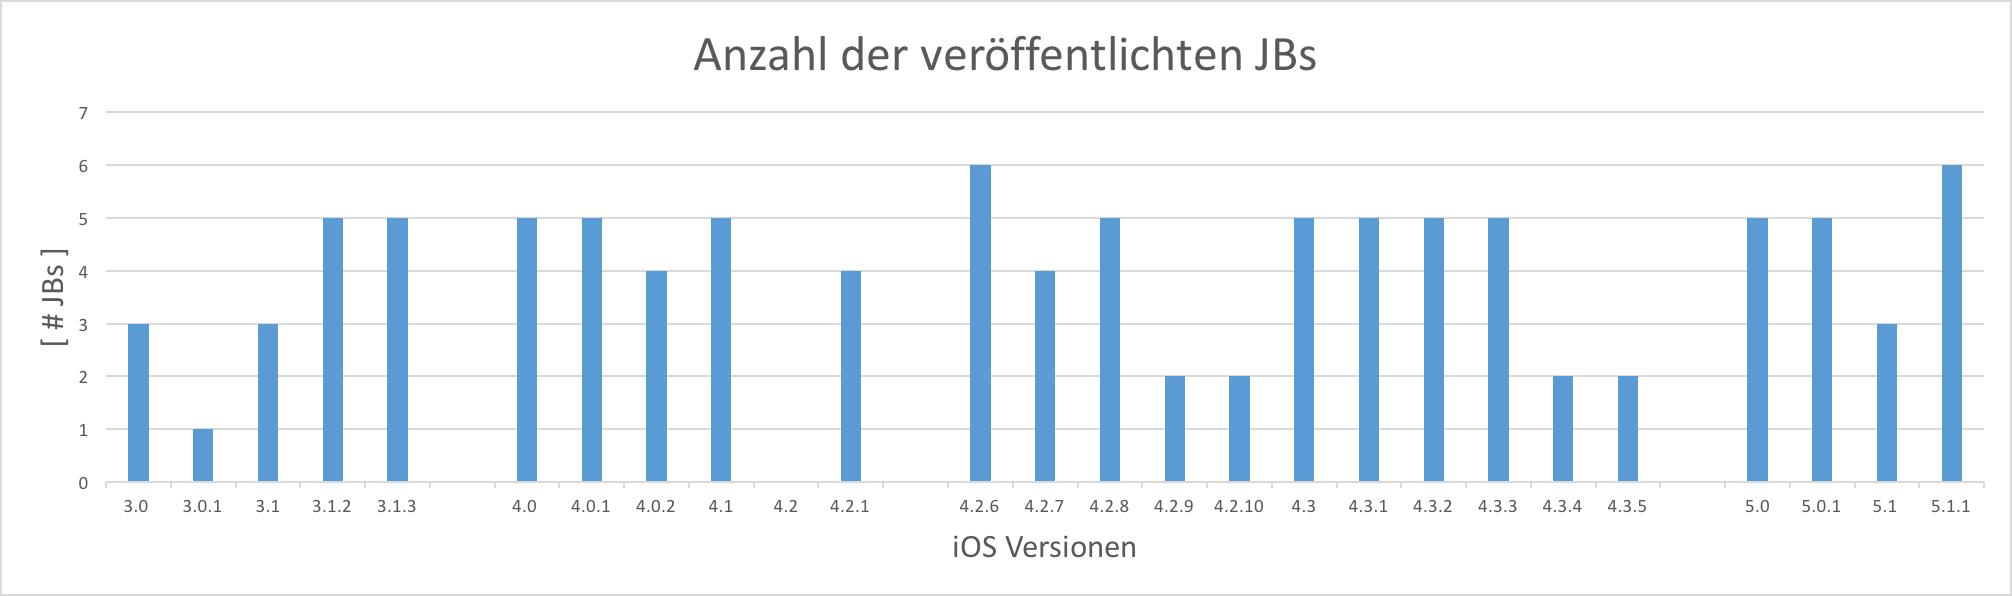
\includegraphics[scale=0.5]{Bilder/iOSJB1.png}
        \caption{Anzahl der veröffentlichten untethered JBs pro iOS \newline Version 3.x - 5.1.1 \protect\footnotemark}
        \label{fig:AnalyseAnzahliOSJB1}
\end{figure}
%\protect\footnotemark
\footnotetext{Quelle Eigenwerk}

\textbf{Die Abbildungen \ref{fig:AnalyseAnzahliOSJB1} und \ref{fig:AnalyseAnzahliOSJB2} zeigen,} dass die Anzahl der veröffentlichten JB-Tools ab der iOS Version 7.0 massiv rückgängig sind. Es wurden nur mehr ein oder zwei JB-Tools pro iOS Version der Öffentlichkeit zur Verfügung gestellt. 

\begin{figure}[htbp!]
        \centering
                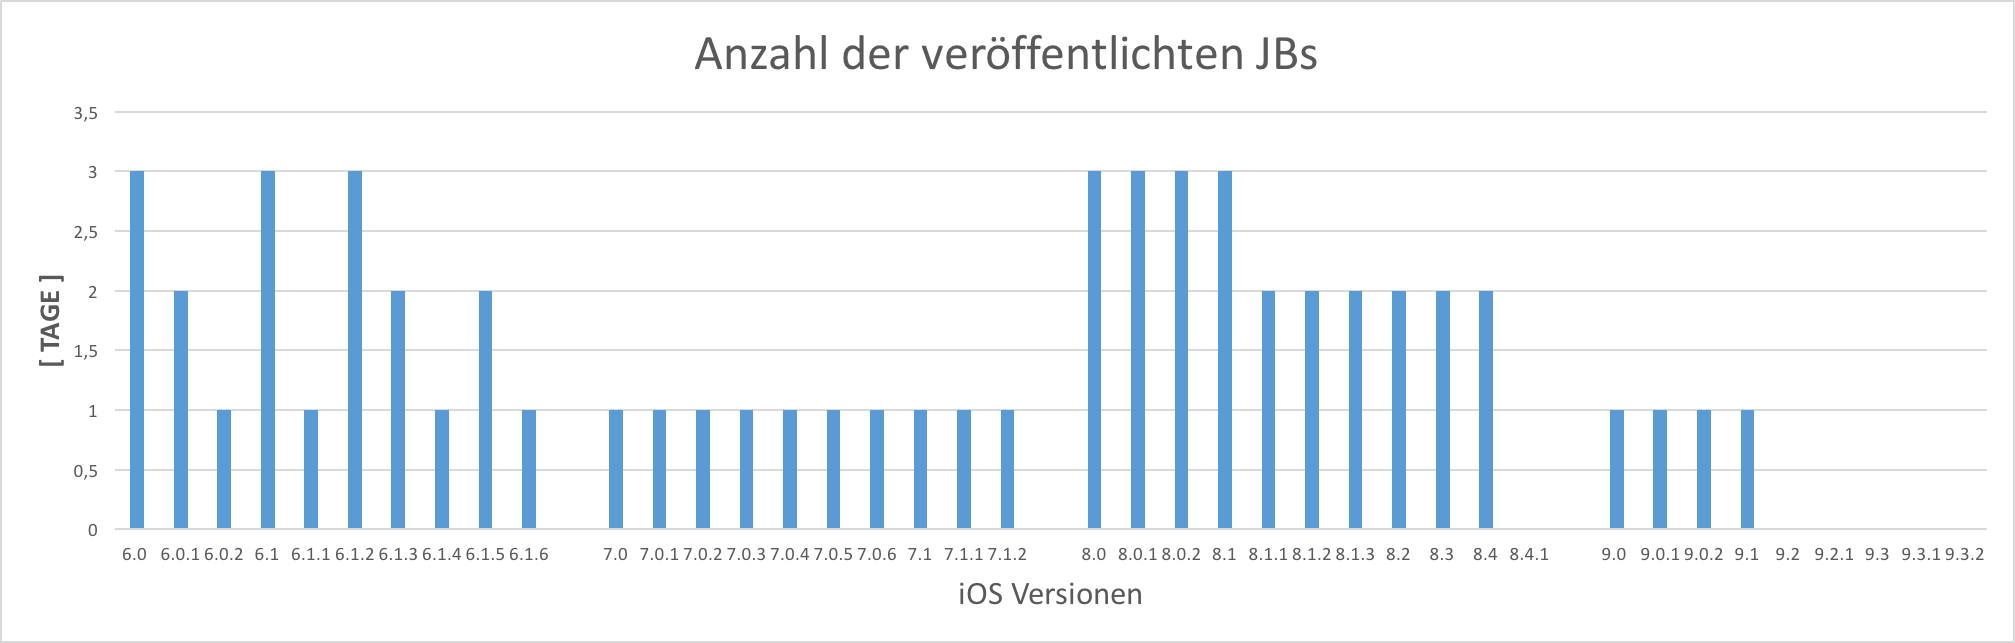
\includegraphics[scale=0.5]{Bilder/iOSJB2.png}
        \caption{Anzahl der veröffentlichten untethered JBs pro iOS \newline Version 6.x - 9.x.x \protect\footnotemark}
        \label{fig:AnalyseAnzahliOSJB2}
\end{figure}
%\protect\footnotemark
\footnotetext{Quelle Eigenwerk}

\paragraph{Ergebnisse:} Anhand der aufbereiteten Daten kann die Konklusion gezogen werden, dass die Sicherheit und die Vertrauenswürdigkeit der iOS Produkte mit steigender iOS Version zunimmt. Dieser Schluss ist darauf begründet, dass die Anzahl der Tage, die benötigt wurden, um einen JB zur Verfügung zu stellen, eine steigende Tendenz aufweisen. Der letzte untethered JB wurde Anfang Dezember 2015 veröffentlicht.
Im Zeitraum von Dezember 2015 bis Juli 2016 wurden sechs weitere iOS Sicherheitsupdates von Apple publiziert. In diesen 243 Tagen (per 18.07.2016) wurden der Öffentlichkeit keine neuen JBs zur Verfügung gestellt.\par 
Ein weiterer Anhaltspunkt für die Steigerung der Sicherheit ist, dass die Anzahl der Softwareentwickler(Hacker) die einen funktionsfähigen Jailbreak entwickeln können, sinkt  (siehe Abb. \ref{fig:AnalyseAnzahliOSJB1} und \ref{fig:AnalyseAnzahliOSJB2}). \par 

Es muss darauf hingewiesen werden, dass Apple seine Strategie in Bezug auf die JB-Community geändert hat. In der Vergangenheit hat Apple versucht, gegen JBs gerichtlich vorzugehen, allerdings mit begrenztem Erfolg (\textit{\glqq Klage gegen George Hotz alias Geohot\grqq{}}). Apple hat vor einigen Jahren damit begonnen, namhafte iOS Hacker anzustellen, unter anderem \textit{\glqq Comex\grqq}, den Entwickler von \textit{\glqq JailbreakMe\grqq}. Dies bringt zwei Vorteile für Apple mit sich. Erstens, die Hacker kennen das mobile Betriebssystem und die Schwächen dieses genauer als viele interne Apple Entwickler.  Zweitens, die JB-Community verliert ein aktives Mitglied. Sehr viel schwerwiegender ist allerdings, dass durch den ehemaligen Hacker auch einige Zero-Day Bugs an Apple gemeldet wurden.\par
Seit dem Jahr 2015 ist der kommerzielle Aspekt in diesem Zusammenhang nicht außer Acht zu lassen. Angefangen vom Preisgeld, welches auf ein JB der iOS Version 9.x ausgesetzt wurde, bis hin zu Prämien für Zero-Day Bugs. Dies hat meiner Ansicht nach einen großen Einfluss auf die Dauer der Veröffentlichung der JBs. Die markanten Ausreißer in den Metriken, ab der iOS Version 9.1, beruhen meinen Analysen nach auf dem kommerziellen Faktor. 
%------------------------------------------------------------------------------
%------------------------------ 
\section{Welche Auswirkung haben die von Apple eingeführten Sicherheitsupdates auf die Sicherheit des Systems?}
\label{sec:Frage2}
%------------------------------------------------------------------------------
%------------------------------ 
%\subsection{iOS Sicherheitsmechanismen}
%\label{sec:Frage2SecMechanismen}
% 
%\begin{table}[htp!]
%    \begin{center}
%        \begin{tabular}{|l|l|l|l|} \hline
%            \textbf{Sicherheitsmechanismus} & \textbf{iOS 2.0} & \textbf{iOS 4.3} & \textbf{iOS 8.0} \\ \hline
%             Anzahl behobener Fehler & nA & 12 & 48\\ \hline
%             MAC & 8 & - & - \\ \hline
%             JIT & 8 & 85 & - \\ \hline
%             ASLR & - & 85 & - \\ \hline
%             verpflichtende Datenverschlüsselung & - & - & 35 \\ \hline
%             verpflichtende Datenverschlüsselung & - & - & 73\\ \hline
%        \end{tabular} 
%        \caption{Auflistung Sicherheitsmechanismus}
%        \label{tab:SecMechanismBugs}
%    \end{center}
%\end{table}

%------------------------------------------------------------------------------
%------------------------------ 
\subsection{iOS Sicherheitsupdates  (G1.2)}
\label{sec:Frage2SecUpdate}

In diesem Kapitel wird auf die Wechselbeziehung zwischen der Sicherheit des iOS Device und den JBs, in Abhängigkeit der Hypothese H1 eingegangen. Im Detail wird die Historie einzelner JB-Tools betrachtet. 

\begin{table}[hp!]
    \begin{center}
        \begin{tabular}{| p{20mm} | p{12mm} | p{17mm} | p{12mm} | p{32mm} | p{22mm} | p{15mm} |} \hline
             \textbf{Datum iOS} & \textbf{iOS} & \textbf{\# Bugs} & \textbf{\# JB Bugs} & \textbf{JB-Tool} & \textbf{JB Datum} & \textbf{\# Tage bis JB} \\ \hline 
            10.02.2011 & 4.2.6 &  - & -  & JailbreakMe 3.0 & 02.06.2011 & 112 \\ \hline
             09.03.2011 & 4.3 & 12 & 0 & JailbreakMe 3.0 &	02.06.2011 & 85 \\ \hline
             25.03.2011 & 4.3.1 &  - & - & JailbreakMe 3.0 & 02.06.2011 & 69 \\ \hline
            14.04.2011 & 4.2.7 &  4 & 0 & JailbreakMe 3.0 & 02.06.2011 & 49 \\ \hline
             15.04.2011 & 4.3.2 & 5 & 0 & JailbreakMe 3.0 & 02.06.2011 & 48 \\ \hline
             04.05.2011 & 4.2.8 &  - & - & JailbreakMe 3.0 & 02.06.2011 & 29 \\ \hline
            \textbf{04.05.2011} & \textbf{4.3.3} &  - & -  & \textbf{JailbreakMe 3.0} & \textbf{02.06.2011} & \textbf{29} \\ \hline
            15.07.2011 & 4.3.4 &  1 & 2	 & - & - & - \\ \hline
        \end{tabular} 
        \caption{Analyse des JB-Tools JailbreakMe 3.0 (vgl. \cite{Apple[7]}) \protect\footnotemark }         
        \label{tab:AnalyseJailbreakMe3.0}
    \end{center}
\end{table}
\footnotetext{Quelle Eigenwerk}
%\footnotetext{Quelle Eigenwerk, Informationen\url{https://support.apple.com/de-de/HT204611}}
%\footnote{\label{foot:iOS2011-2012}{\url{https://support.apple.com/de-de/HT204611}}}

\paragraph{JailbreakMe 3.0} ist ein \textit{\glqq webbasierter Userland Exploit\grqq{}} und wurde am 02.06.2011 veröffentlicht. Dieser untethered Jailbreak wurde für die iOS Version 4.3.3 bereitgestellt. Es konnten aber mit diesem Exploit auch die iOS Versionen 4.2.6 bis 4.3.3 (siehe Tab.\ref{tab:AnalyseJailbreakMe3.0})  \textit{\glqq gejailbreaked\grqq{}} werden. 
Es wurde ein Fehler im CoreGraphik Framework ausgenutzt, welcher es erlaubte, im Zusammenhang mit dem Lesen eines PDFs einen beliebigen Code auszuführen. Der IOMobileFrameBuffer hatte einen weiteren Softwarefehler, welcher es den JailbreakMe 3.0 Exploit ermöglichte, Systemprivilegien zu erhalten. Beide Bugs wurden in der iOS Version 4.3.4 \footnote{\label{foot:iOS4.3.4}{\url{https://support.apple.com/de-de/HT202272}}} geschlossen. Ab der iOS Version 4.3.4 ist dieser JB nicht mehr funktionsfähig.
 
\paragraph{Ergebnisse:} Interessant an den Daten der Tabelle \ref{tab:AnalyseJailbreakMe3.0} ist, dass in einem Zeitraum von 112 Tagen sechs iOS Sicherheitsupdates von Apple zur Verfügung gestellt wurden. In diesen sechs Updates wurden insgesamt 21 Bugs behoben. Das Schließen dieser Sicherheitslücken hatte keine Auswirkung auf den später veröffentlichten JB. Dieses Verhalten spiegelt sich in allen analysierten JB-Tools wieder. \par  
Am 15.07.2011 wurde das iOS Sicherheitsupdate 4.3.4 zum Download zur Verfügung gestellt. In diesem Update wurden insgesamt drei Sicherheitslücken von Apple geschlossen. JailbreakMe 3.0 verwendete zwei von diesen Bugs, und somit war der JB für alle weiteren iOS Versionen unterbunden. Dies läßt vermuten, dass Apple die JB-Tools \textit{\glqq Reverse Engineered\grqq{}} und gezielt Sicherheitsupdates, zum Unterbinden dieser, zur Verfügung stellt. Apple benötigte 43 Tage um ein Update bereitzustellen. Dies zeigt, dass die JBs einen direkten Einfluss auf die Sicherheit und Vertrauenswürdigkeit des iOS Systems haben, da Apple anhand der in der Analyse gefundenen Bugs, Sicherheitsupdates zur Verfügung stellt. \par 

\begin{table}[hp!]
    \begin{center}
        \begin{tabular}{| p{15mm} | p{20mm} | p{17mm} | p{12mm} | p{20mm} | p{22mm} | p{15mm} |} \hline
            \textbf{iOS} & \textbf{Datum iOS} & \textbf{\# Bugs} & \textbf{\# JB Bugs} & \textbf{JB-Tool} & \textbf{JB Datum} & \textbf{\# Tage bis JB} \\ \hline 
7.1 & 10.03.2014 & 20 & 4 & Pangu & 23.6.2014 & 105 \\ \hline
\textbf{7.1.1} & \textbf{22.04.2014} & \textbf{4} & \textbf{0} & \textbf{Pangu} & \textbf{23.6.2014} & \textbf{62} \\ \hline
7.1.2 & 30.06.2014 & 18 & 0 & Pangu & 23.6.2014 & -7 \\ \hline
 & & & & & & \\ \hline
8.0 & 17.09.2014 & 44 & 4 & Pangu8 & 22.10.2014 & 35 \\ \hline
8.0.1 & 24.09.2014 & - & - & Pangu8 & 22.10.2014 & 28 \\ \hline
8.0.2 & 25.09.2014 & - & - & Pangu8 & 22.10.2014 & 27 \\ \hline
\textbf{8.1} & \textbf{20.10.2014} & \textbf{5} & \textbf{0} & \textbf{Pangu8} & \textbf{22.10.2014} & \textbf{2} \\ \hline
8.1.1 & 17.11.2014 & 5 & 3 & - & - & - \\ \hline
 & & & & & & \\ \hline
9.0& 16.09.2015 & 71 & 1 & Pangu9 & 14.10.2015 & 28  \\ \hline
\textbf{9.0.1} & \textbf{23.09.2015} & \textbf{-} & \textbf{-} & \textbf{Pangu9} & \textbf{14.10.2015} & \textbf{21}\\ \hline
9.0.2 & 30.09.2015 & 1 & 0 & Pangu9 & 14.10.2015 & -14 \\ \hline
9.1(32 Bit) & 21.10.2015 & 25 & 2 & Pangu9 & 14.10.2015 & -  \\ \hline
		 & & & & & & \\ \hline				
\textbf{9.1(64 Bit)} & \textbf{21.10.2015} & \textbf{25} & \textbf{2} & \textbf{Pangu9} & \textbf{11.3.2016} & \textbf{142}  \\ \hline
9.2 & 08.12.2015	 & 27 & 3 & - & - & - \\ \hline		
     \end{tabular} 
        \caption{Analyse des JB-Tools Pangu (vgl. \cite{Apple[7]}) \protect\footnotemark}
        \label{tab:AnalysePangu}
    \end{center}
\end{table}
\footnotetext{Quelle Eigenwerk}
%\footnotetext{\url{https://support.apple.com/de-de/HT201222}}

\paragraph{Das JB-Team Pangu} veröffentlichte in den letzten zwei Jahren JBs für drei Major iOS Versionen. Bevor das Team Pangu ihren ersten JB veröffentlichte, nahmen die Member des Teams an einem iOS Exploitation Training von \textit{\glqq Stefan Essers\grqq{}} teil \footnote{\url{https://www.sektioneins.de/en/trainings/iosexploitation.html}}. Zu Kontroversen führte dieser JB, da dieser auf dem im Training vorgeführten Kernel Exploits beruhte.\par
Bis zum heutigen Datum (18.07.2016) wurden vom Pangu Team vier unterschiedliche JB Versionen veröffentlicht. Mit diesen vier JBs können zwölf iOS Versionen \textit{\glqq gejailbreaked\grqq{}} werden (siehe Tab.\ref{tab:AnalysePangu}).

Die Tabelle \ref{tab:AnalysePangu} zeigt dasselbe Muster wie in dem zuvor analysierten JB-Tool JailbreakMe 3.0. Mit einer Ausnahme verhinderte das nächste iOS Sicherheitsupdate 9.0.2 nicht den JB, der vierzehn Tage zuvor veröffentlicht wurde. \par 
Dem Pangu Team gelang es, als erstes JB-Team, nach 142 Tagen, einen JB für die iOS Version 9.1 für die 64 Bit Prozessor-Architektur zu entwickeln.

\paragraph{Ergebnisse:}  Die iOS Version 7.1.2 ist das letzte verfügbare Sicherheitsupdate für das iPhone 4. Diese iOS Version ist als nicht sicher einzustufen. Dadurch ist das iPhone 4 als unsicher und nicht vertrauenswürdig zu beurteilen.\par 
Interessant ist auch, dass das iOS Sicherheitsupdate 8.1.1 drei Softwarefehler behebt, die vom JB-Tool Pangu8 verwendet wurden. Nach 26 Tagen wurden die Sicherheitslücken geschlossen, die den JB Pangu8 ermöglichten. Das iOS Sicherheitsupdate 8.1.1 hatte aber nur einen geringen Einfluss auf das JB-Tool TaiG. Dies zeigt deutlich, dass Apple gezielt Bugs von einzelnen JB-Tools schließt. 

Apple schloss in der iOS Version 9.0 72 Sicherheitslücken und das JB-Team Pangu benötigte 28 Tage, um diese Version zu \textit{\glqq jailbreaken\grqq{}}. Die iOS Version 9.2 beendete nach 55 Tagen die Funktionsfähigkeit des JB-Tools Pangu9 . Daraus resultiert, dass die Anzahl an geschlossenen Sicherheitsfehlern keinen direkten Einfluss auf den JB haben.

\begin{table}[htp!]
    \begin{center}
        \begin{tabular}{| p{10mm} | p{22mm} | p{17mm} | p{12mm} | p{18mm} | p{22mm} | p{15mm} |} \hline
            \textbf{iOS} & \textbf{Datum iOS} & \textbf{\# Bugs} & \textbf{\# JB Bugs} & \textbf{JB-Tool} & \textbf{JB Datum} & \textbf{\# Tage bis JB} \\ \hline 
8.0 & 17.09.2014 & 44 & 4 & TaiG & 29.11.2014 & 73  \\ \hline
8.0.1 & 24.09.2014	& - & - & TaiG & 29.11.2014 & 66 \\ \hline
8.0.2 & 25.09.2014 & - & -  & TaiG & 29.11.2014 & 65  \\ \hline
8.1 & 20.10.2014 & 5 & 0 & TaiG & 29.11.2014 & 40  \\ \hline
\textbf{8.1.1} & \textbf{17.11.2014} & \textbf{5} & \textbf{3} & \textbf{TaiG} & \textbf{29.11.2014} & \textbf{12}  \\ \hline
 & & & & & & \\ \hline						
\textbf{8.1.2} & \textbf{09.12.2014} & \textbf{1} & \textbf{0} & \textbf{TaiG v2} & \textbf{08.03.2015} & \textbf{89}  \\ \hline
	 & & & & & & \\ \hline						
8.1.3 & 27.01.2015 & 16 & 5 & TaiG v3 & 23.06.2015 & 147  \\ \hline
8.2  & 09.03.2015 & 5 & 1 & TaiG v3 & 23.06.2015 & 106 \\ \hline
\textbf{8.3} &  \textbf{08.04.2015} & \textbf{40} & \textbf{1} & \textbf{TaiG v3} & \textbf{23.06.2015} & \textbf{103}  \\ \hline
		 & & & & & & \\ \hline					
\textbf{8.4} &  \textbf{30.06.2015} & \textbf{25} & \textbf{0} & \textbf{TaiG v4} & \textbf{01.07.2015} & \textbf{1}  \\ \hline
8.4.1 & 13.08.2015 & 35 & 9 & - & - & -   \\ \hline
        \end{tabular} 
        \caption{Analyse des JB-Tools TaiG (vgl. \cite{Apple[7]}) \protect\footnotemark}
        \label{tab:AnalyseTaig}
    \end{center}
\end{table}
\footnotetext{Quelle Eigenwerk}
%\footnotetext{\url{https://support.apple.com/de-de/HT205762}}

\paragraph{TaiG} zeigt wie kein anderes JB-Tool, wie sehr Apple und die JB-Community Katz und Maus spielen  (siehe Tab. \ref{tab:AnalyseTaig}). Apple antwortete innerhalb weniger Tage mit einem Update, welches das JB schließt. Das JB-Team TaiG veröffentlichte für jedes iOS Sicherheitsupdate ein neues JB, bis am Ende Apple das iOS Sicherheitsupdate 8.4.1 veröffentlichte. In diesem Update werden acht Softwarefehler geschlossen, auf dem der TaiG JB aufbaute. 
 
Das iOS Sicherheitsupdate 8.1.2 wurde zehn Tage nach dem JB-Tool TaiG veröffentlicht und behob die Sicherheitslücken der iOS Version 8.1.1. Dadurch funktionierte der TaiG JB in der iOS Version 8.1.2 nicht mehr.

Das JB-Tool TaiG v2 war schon bei seiner Veröffentlichung obsolet, da das iOS Sicherheitsupdate 8.1.3 schon zuvor veröffentlicht wurde. In diesem wurden fünf Sicherheitslücken geschlossen, auf denen das JB-Tool TaiG v2 aufbaute.
Die Sicherheitslücken, die für das JB-Tool TaiG v3 verwendet wurden, wurden teilweise nach sieben Tagen im iOS Sicherheitsupdate 8.4 geschlossen. In diesem iOS Sicherheitsupdate wurden 25 Bugs geschlossen, aber schon nach einem Tag wurde das JB-Tool TaiG v4 veröffentlicht. Die iOS Version 8.4.1 beendete nach 43 Tagen die Funktionsfähigkeit des JB TaiG v4.

\begin{table}[htp!]
    \begin{center}
        \begin{tabular}{| p{10mm} | p{40mm} | p{17mm} |} \hline
            \textbf{iOS} & \textbf{JB-Tool} & \textbf{\# Tage} \\ \hline 
                4.3.4 & JailbreakMe 3.0 & 43 \\ \hline
                8.1.1 & Pangu8 & 26 \\ \hline
                9.2 & Pangu9 & 55 \\ \hline
                8.1.2 & TaiG & 10  \\ \hline
                 8.1.3 & TaiG v2 & - \\ \hline
                  8.4 & TaiG v3 & 7  \\ \hline
                  8.4.1 & TaiG v4 & 43  \\ \hline
        \end{tabular} 
        \caption{Apples Reaktionszeiten auf die JBs \protect\footnotemark}
        \label{tab:AppleReaktionszeit}
    \end{center}
\end{table}
\footnotetext{Quelle Eigenwerk}
Im Durchschnitt veröffentlichte Apple nach 37 Tagen ein Sicherheitsupdate, welches die iOS Sicherheitslücken, die für den JB verwendet wurden, schliesst. Die gesamten Daten der Reaktionszeiten sind in der Tabelle \ref{tab:AppleReaktionszeitAll} ersichtlich.  
\newpage
%------------------------------------------------------------------------------
%------------------------------ 
\section{Ergebnis Hypothese H1}
\label{sec:AnalyseHypo}
Die ausgewerteten Daten zeigen, dass die Sicherheit und die Vertrauenswürdigkeit des iOS System mit steigender iOS Version zunimmt. 

\begin{description}
    \item[\parbox{\textwidth} {Dieser Schluss ist darauf begründet, dass}]~\par
    \begin{enumerate}
        \item die Anzahl der veröffentlichten JB-Tools pro iOS Version sinkt,
        \item die Anzahl der Tage, die benötigt werden, um ein JB zu veröffentlichen, markant zunimmt. Vor allem ab der iOS Release 9.x;
        \item und die Anzahl der geschlossenen Sicherheitslücken pro Major Release eine aufsteigende Tendenz aufweist (siehe Abb. \ref{fig:SecUpdateMajor}).
    \end{enumerate}
\end{description} 

%Die Anzahl der Tage die bis zur Veröffentlichung eines JB benötigt werden, hängen noch von anderen Faktoren ab.
\begin{description}
    \item[\parbox{\textwidth} {Neben der Sicherheit der iOS Version haben folgende Faktoren einen Einfluss auf die Veröffentlichungsdauer eines JBs}]~\par
    \begin{enumerate}
        \item die mangelnde Kontinuität der JB-Teams,
        \item der kommerzielle Faktor,
        \item und dass die JB-Community ihre JBs zurückhält, wenn Apple bekannt
gibt, dass eine neue Major Release veröffentlicht wird.
    \end{enumerate}
\end{description}
Diese Faktoren können nicht aus den Daten, auf denen diese Arbeit aufbaut, extrahiert werden und deshalb kann die Hypothese H1 (siehe Kap. 1.4.3) nur teilweise bestätigt werden.

\begin{figure}[hp!]
        \centering
                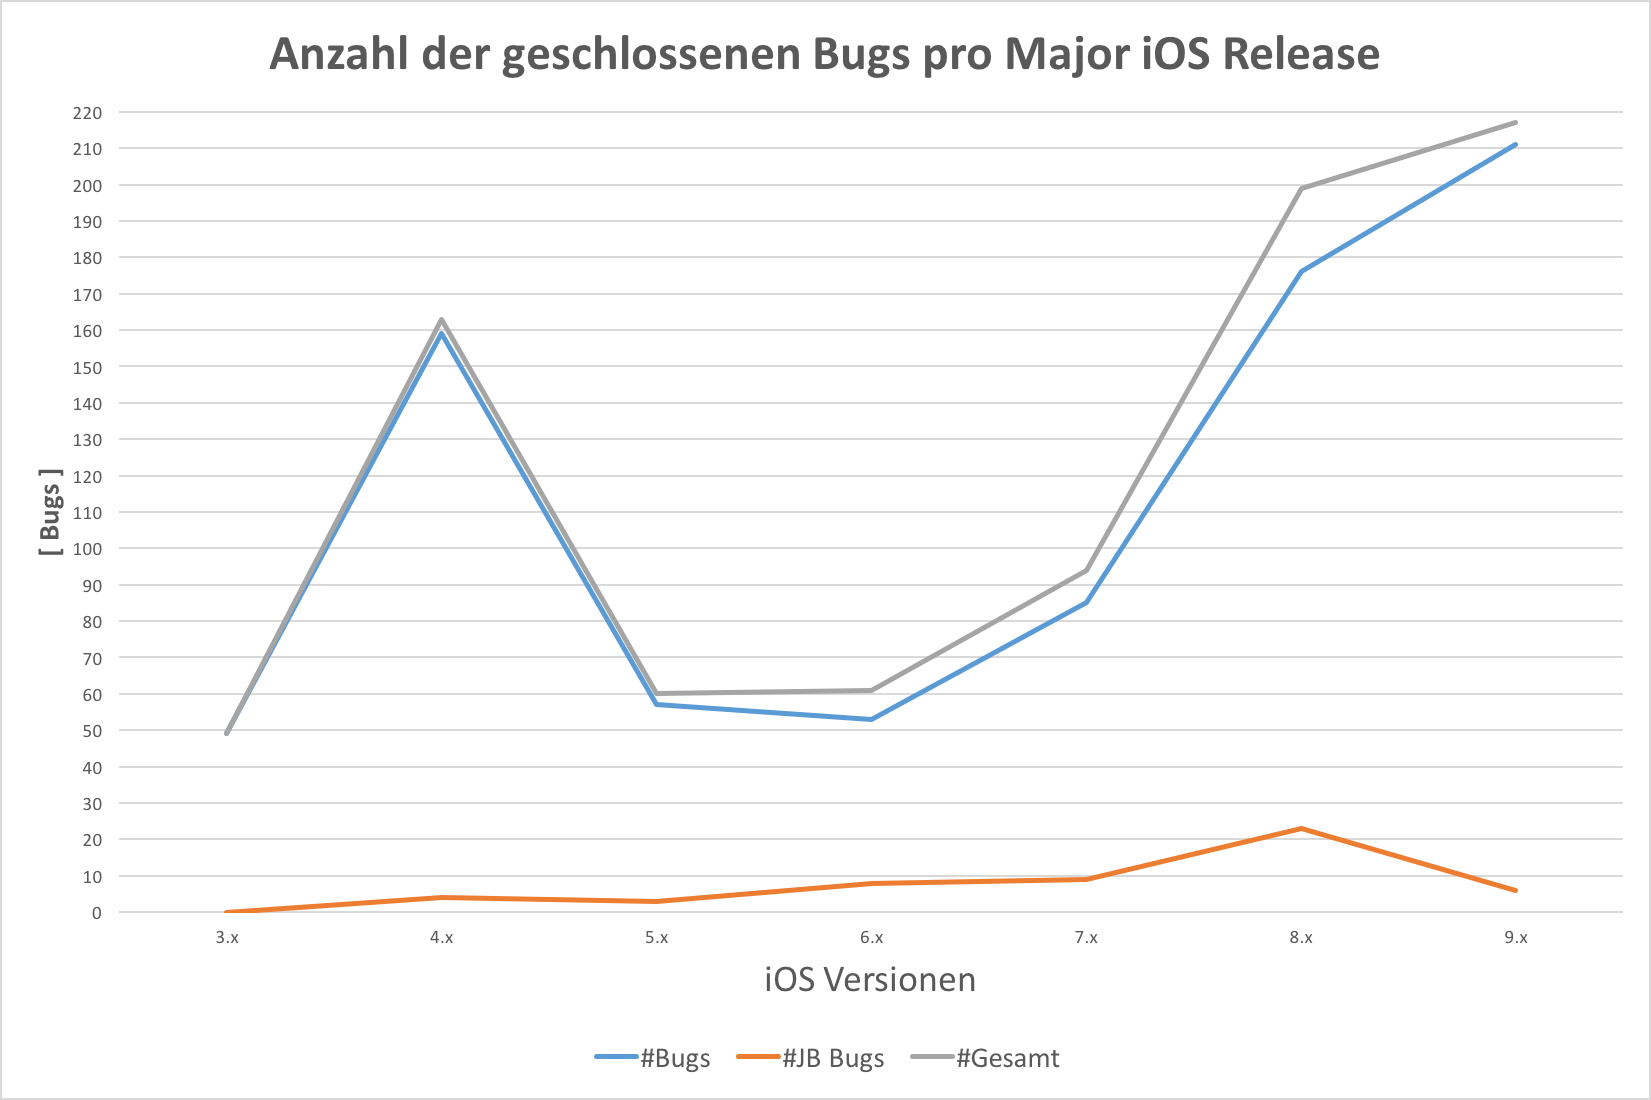
\includegraphics[scale=0.42]{Bilder/SecUpdateMajor.png}
        \caption{Anzahl der geschlossenen Bugs pro iOS Major Release \newline (vgl. \cite{Apple[7]}) \protect\footnotemark}
        \label{fig:SecUpdateMajor}
\end{figure}
\footnotetext{Quelle Eigenwerk}
\newpage

\section{Ergebnis Ziel G1.1}
\label{sec:AnalyseG11}
% G1.1: Erstes abgeleitetes Ziel ist es, einen Zusammenhang zwischen der Sicherheit und der Vertrauenswürdigkeit des iOS Device und der verwendeten Hardware der iOS Geräte herzustellen.
 Die Hardware der iOS Produkte spielt bei der Sicherheit des iOS Device nur eine begrenzte Rolle. Die Daten in den Kapiteln \ref{sec:Frage1iOSVersion} und \ref{sec:Frage1SecureEnclave} zeigen diesen Sachverhalt ganz klar.\par  
Die Secure Enclave verbesserte die Vertraulichkeit des iOS Device, da die gesamten kryptographischen Verfahren für die File Keys, die Daten für den FingerPrint und vieles mehr in der Trust Zone des AMD Prozessors gespeichert werden. \par
Zu diesem Thema muss noch gesagt werden, dass die iOS Produkte ein in sich geschlossenes System sind. Dies bedeutet, der User kann weder die Hardware des Systems noch das Betriebssystem verändern. Alle Komponenten passen perfekt zueinander und sind aufeinander abgestimmt. Das iOS wurde für die Hardware des iOS Devices entwickelt und abgestimmt. Dies bringt Vorteile gegenüber anderen mobilen Betriebssystemen wie z.B. Android.  

\begin{description}
    \item[\parbox{\textwidth} {Zum heutigen Zeitpunkt sind sieben iPhones als nicht sicher einzustufen}]~\par
    \begin{enumerate}
        \item iPhone - letzte unterstützte iOS Version 3.1.3
        \item iPhone 3G - letzte unterstützte iOS Version 4.2.1
        \item iPhone 3GS - letzte unterstützte iOS Version 6.1.6
        \item iPhone 4 - kein Coprozessor mit Secure Enclave
        \item iPhone 4s - kein Coprozessor mit Secure Enclave
        \item iPhone 5 - kein Coprozessor mit Secure Enclave
        \item iPhone 5c - kein Coprozessor mit Secure Enclave
    \end{enumerate}
\end{description} 
 
\section{Ergebnis Ziel G1.2}
\label{sec:AnalyseG12}

%G1.2: Zweites abgeleitetes Ziel dieser Arbeit ist es, einen Zusammenhang zwischen der Sicherheit und der Vertrauenswürdigkeit des iOS Device und der installierten iOS Software herzustellen.

Die erhobenen Daten zeigen, dass die Sicherheit des Systems neben dem verwendeten Passcode, der iOS Konfiguration, dem iOS selbst, noch von einem weiteren Faktor massiv abhängt: \textbf{den regelmäßigen Sicherheitsupdates}.  
\begin{description}
    \item[\parbox{\textwidth} {Bei der Konfiguration sind folgende Konfigurationsparameter anzuführen}]~\par
    \begin{itemize}
       \item die Anzahl der Stellen des Passcodes
       \item die Aktivierung des Parameters \textit{\glqq Daten löschen\grqq{}}. Das hat zur Folge, dass nach zehn falschen Eingaben des Passcodes alle Daten des iOS Device gelöscht werden.
    \end{itemize}
\end{description} 

Apple veröffentlichte bis zum heutigen Datum (18.7.2016) für die iOS Major Release 9.x neun Sicherheitsupdates. Diese Sicherheitsupdates schlossen insgesamt 217 Bugs. Sechs dieser Bugs wurden für das JB Pangu verwendet.  Seit der iOS Version 3.x wurden insgesamt 843 Softwarefehler in 49 Sicherheitsupdates geschlossen. 55 dieser Softwarefehler wurden von JB-Tools verwendet. Eine genaue Auflistung der Daten ist in den Abbildungen \ref{fig:AnalyseiOSSicherheitsupdate3}, \ref{fig:AnalyseiOSSicherheitsupdate5}, \ref{fig:AnalyseiOSSicherheitsupdate5}, \ref{fig:AnalyseiOSSicherheitsupdate7}, \ref{fig:AnalyseiOSSicherheitsupdate8} und \ref{fig:AnalyseiOSSicherheitsupdate9} ersichtlich.

Die Daten lassen vermuten, dass Apple gezielt JB-Tools „Reverse Engineering“ und die für das JB verwendeten Sicherheitslücken der iOS Version schließt.

\section{Ergebnis Ziel G1}
\label{sec:AnalyseG1}

Das iOS Device gehört zu den sichersten mobilen Geräten auf dem freien Markt. Die iOS Update-Funktionalität ist im iOS Betriebssystem integriert. Der User wird in regelmäßigen Abständen daran erinnert, dass eine neue iOS Version zur Verfügung steht. Somit wird der User aktiv animiert, die iOS Version auf seinem Gerät aktuell zu halten. Bei Android ist der OS Update-Mechanismus vom Gerätehersteller abhängig. Wenn der Hersteller dieses Feature unterstützt, dann sind die Sicherheitsupdates meist zeitverzögert, da der Hersteller seine eigene Android Versionen zur Verfügungen stellt. Unterstützt der Hersteller die automatischen Sicherheitsupdates nicht, so ist der User selbst für die Betriebssystem-Aktualisierung verantwortlich (siehe Abb. \ref{fig:VergleichUpdateiOSAndroid}).\par
 \begin{figure}[hp!]
        \centering
                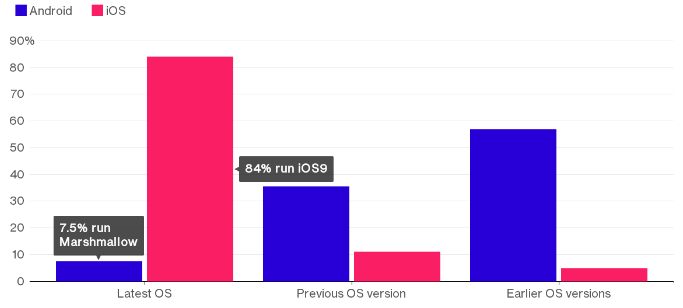
\includegraphics[scale=0.8]{Bilder/updatesiOSAndroid.PNG}
        \caption{OS Update-Vergleich zwischen iOS und Android (Quelle \cite{ANDROID[1]})}
        \label{fig:VergleichUpdateiOSAndroid}
\end{figure}

Im Vergleich zu Android veröffentlicht Apple weit mehr Sicherheitsupdates pro Jahr. Daraus kann einerseits geschlossen werden, dass die iOS Versionen aufgrund der Mehrzahl an Bugs als unsicherer einzustufen sind. Die andere Sichtweise ist, dass unter iOS mehr Codeanalysen durchgeführt werden. Ich schließe mich der zweiten Aussage an, da aufgrund der JBs mehr Aufmerksamkeit auf die zeitnahen Sicherheitsupdates gelegt wird. Es würde zu einem Imageverlust führen, wenn Sicherheitslücken zu lange ausgenutzt werden können. \par

\begin{description}
    \item[\parbox{\textwidth} {Auch in Bezug auf die Sicherheitsmechanismen hat Apple weitere Vorteile gegenüber Android}]~\par
    \begin{enumerate}
        \item Apple verwendet MAC und nicht wie Android DEP (siehe Kap. \ref{sec:MAC})
        \item Es können nur Apps am iOS Device installiert werden, die mit einen Apple Zertifikat signiert wurden. Unter Android können selbstsignierte Apps installiert werden, sowie bei iOS Device mit JB.
        \item Android überprüft die Apps automatisiert, während bei Apple diese von Apple Mitarbeitern geprüft werden, bevor die Apps im iTunes Store heruntergeladen werden können.  
    \end{enumerate}
\end{description} 

Ein interessantes Detail ist noch anzuführen. Die im Laufe der Jahre eingeführten Sicherheitsmechanismen wie zum Beispiel, ALSR, MAC und Sandbox, hatten keinen markanten Einfluss auf die Anzahl an Tagen, die benötigt wurden, um ein JB zu veröffentlichen. In den Abb. 5.2 und 5.3 gibt es keine Ausreißer in den Metriken.\par  
Erwartet hätte ich mir, dass zwischen der iOS Version 2.0 und 4.3 die Anzahl an Tagen, bis ein JB veröffentlicht wurde, enorm ansteigt.  Es gab nur eine markante Stelle. Die iOS Version 3.1.2 zeigt einen massiven Anstieg der Anzahl an Tagen, die benötigt wurden, um die untethered JBs \textit{\glqq JailbreakMe 2.0\grqq{}} und \textit{\glqq Spirit\grqq{}} zu veröffentlichen. Dies ist aber darauf zurückzuführen, dass diese beiden Tools neu entwickelt wurden. Das JB-Tool \textit{\glqq sn0wbreeze 1.1\grqq{}} konnte nach 95 Tagen einen JB für diese iOS Version zur Verfügung stellen.\par
 
In Bezug auf JBs kann gesagt werden, dass ein installierter JB die Sicherheit und Vertrauenswürdigkeit des Systems reduziert, da Sicherheitsmechanismen von Apple eingeschränkt und/oder deaktiviert werden. Der normale User ist sich über diese Konsequenzen nicht im Klaren und verfügt meistens nicht über das Wissen, das Device wieder sicher zu machen.

